\documentclass[aps,prb,twocolumn,superscriptaddress,floatfix,longbibliography]{revtex4-2}

\usepackage[utf8]{inputenc}
\usepackage[spanish]{babel}
\usepackage{graphicx}
\usepackage{amsmath}
\usepackage{subcaption}
\usepackage{wrapfig} 
\usepackage[export]{adjustbox}

\usepackage{amsmath,amssymb} % math symbols
\usepackage{bm} % bold math font
\usepackage{graphicx} % for figures
\usepackage{comment} % allows block comments
\usepackage{textcomp} % This package is just to give the text quote '
\usepackage{listings} %para agregar código

%\usepackage{ulem} % allows strikeout text, e.g. \sout{text}

\usepackage[spanish]{babel}

\usepackage{enumitem}
\setlist{noitemsep,leftmargin=*,topsep=0pt,parsep=0pt}

\usepackage{xcolor} % \textcolor{red}{text} will be red for notes
\definecolor{lightgray}{gray}{0.6}
\definecolor{medgray}{gray}{0.4}

\usepackage{hyperref}
\hypersetup{
colorlinks=true,
urlcolor= blue,
citecolor=blue,
linkcolor= blue,
bookmarks=true,
bookmarksopen=false,
}

% Code to add paragraph numbers and titles
\newif\ifptitle
\newif\ifpnumber
\newcounter{para}
\newcommand\ptitle[1]{\par\refstepcounter{para}
{\ifpnumber{\noindent\textcolor{lightgray}{\textbf{\thepara}}\indent}\fi}
{\ifptitle{\textbf{[{#1}]}}\fi}}
%\ptitletrue  % comment this line to hide paragraph titles
%\pnumbertrue  % comment this line to hide paragraph numbers

% minimum font size for figures
\newcommand{\minfont}{6}

% Uncomment this line if you prefer your vectors to appear as bold letters.
% By default they will appear with arrows over them.
% \renewcommand{\vec}[1]{\bm{#1}}

%Cambiar Cuadros por Tablas y lista de...
%\renewcommand{\listtablename}{Índice de tablas}
\renewcommand{\tablename}{Tabla}
\renewcommand{\date}{Fecha}

% \graphicspath{ {C:/Users/lupam/Mi unidad/Pablo Chehade/Instituto Balseiro (IB)/Laboratorio Avanzado/Informe/V5/Figures} } %Para importar imagenes desde una carpeta


\lstset{
  basicstyle=\ttfamily\small,
  breaklines=true,
  frame=single,
  numbers=left,
  numberstyle=\tiny,
  keywordstyle=\color{blue},
  commentstyle=\color{green},
  stringstyle=\color{red},
} %Configuración para el bloque de código


\usepackage[bottom]{footmisc} %para que las notas al pie aparezcan en la misma página



\begin{comment}

%Comandos de interes:

* Para ordenar el documento:
\section{Introducción}
\section{\label{sec:Formatting}Formatting} %label para luego hacer referencia a esa sección

\ptitle{Start writing while you experiment} %pone nombre y título al documento dependiendo de si en el header están los comandos \ptitletrue y \pnumbertrue

* Ecuaciones:
\begin{equation}
a^2+b^2=c^2 \,.
\label{eqn:Pythagoras}
\end{equation}

* Conjunto de ecuaciones:
\begin{eqnarray}
\label{eqn:diagonal}
\nonumber d & = & \sqrt{a^2 + b^2 + c^2} \\
& = & \sqrt{3^2+4^2+12^2} = 13
\end{eqnarray}

* Para hacer items / enumerar:
\begin{enumerate}
  \item
\end{enumerate}

\begin{itemize}
  \item
\end{itemize}

* Figuras:
\begin{figure}[h]
    \includegraphics[clip=true,width=\columnwidth]{pixel-compare}
    \caption{}
     \label{fig:pixels}
\end{figure}

* Conjunto de figuras:
(no recuerdo)


* Para hacer referencias a fórmulas, tablas, secciones, ... dentro del documento:
\ref{tab:spacing}

* Para citar
Elementos de .bib
\cite{WhitesidesAdvMat2004}
url
\url{http://www.mendeley.com/}\\

* Agradecimientos:
\begin{acknowledgments}
We acknowledge advice from Jessie Zhang and Harry Pirie to produce Fig.\ \ref{fig:pixels}.
\end{acknowledgments}

* Apéndice:
\appendix
\section{\label{app:Mendeley}Mendeley}

* Bibliografía:
\bibliography{Hoffman-example-paper}

\end{comment}


\begin{document}

% Allows to rewrite the same title in the supplement
\newcommand{\mytitle}{Memorias Asociativas}

\title{\mytitle}

\author{Pablo Chehade \\
    \small \textit{pablo.chehade@ib.edu.ar} \\
    \small \textit{Redes Neuronales, Instituto Balseiro, CNEA-UNCuyo, Bariloche, Argentina, 2023} \\}
    
\maketitle


\section*{Ejercicio 1}



Se calculó la dinámica de una red de Hopfield sin ruido con regla de actualización secuencial y paralela para tamaños de red \( N = 500, 1000, 2000, 4000 \) y para valores de \( \alpha = \frac{p}{N} = 0.12, 0.14, 0.16, 0.18 \), con $p$ número de patrones. En cada red, se realizaron \( p \) simulaciones donde se tomó como condición inicial cada uno de los patrones aleatorios $\xi^\mu$ y se iteró la dinámica hasta converger a un punto fijo \( s_i^{\mu} \). La convergencia fue evaluada mediante la comparación de la configuración de la red en un tiempo grande \( t \) con su estado en \( t+1 \).

En base a los resultados, se calculó la fracción de simulaciones convergidas (\( f_{conv} \)) para la iteración secuencial y paralela variando $N$ y $\alpha$. Los resultados se resumen en las tablas \ref{tab:ej1_f_conv_secuencial} y \ref{tab:ej1_f_conv_paralela}.

% Tabla de f_conv para iteración secuencial
\begin{table}[h]
  \centering
  \caption{Fracción de simulaciones convergidas (\( f_{conv} \)) para iteración secuencial}
  \label{tab:ej1_f_conv_secuencial}
  \begin{tabular}{|c|c|c|c|c|}
  \hline
  \( N \) \ \( \alpha \) & 0.12   & 0.14   & 0.16   & 0.18   \\ \hline
  500            & 1.0000 & 1.0000 & 1.0000 & 1.0000 \\ \hline
  1000           & 1.0000 & 1.0000 & 1.0000 & 1.0000 \\ \hline
  2000           & 1.0000 & 1.0000 & 1.0000 & 1.0000 \\ \hline
  4000           & 1.0000 & 1.0000 & 1.0000 & 1.0000 \\ \hline
  \end{tabular}
\end{table}
  
% Tabla de f_conv para iteración paralela
\begin{table}[h]
  \centering
  \caption{Fracción de simulaciones convergidas (\( f_{conv} \)) para iteración paralela}
  \label{tab:ej1_f_conv_paralela}
  \begin{tabular}{|c|c|c|c|c|}
  \hline
  \( N \) \ \( \alpha \) & 0.12   & 0.14   & 0.16   & 0.18   \\ \hline
  500            & 0.9667 & 0.9143 & 0.7125 & 0.5000 \\ \hline
  1000           & 0.9333 & 0.8643 & 0.4062 & 0.1111 \\ \hline
  2000           & 0.9625 & 0.7071 & 0.2437 & 0.0306 \\ \hline
  4000           & 0.8875 & 0.5250 & 0.0688 & 0.0000 \\ \hline
  \end{tabular}
\end{table}
  

Se observó una completa convergencia $f_{conv} = 1$ en la dinámica secuencial para todos los valores de \( N \) y \( \alpha \). En contraste, la dinámica paralela mostró una disminución progresiva en la convergencia con el aumento de \( \alpha \) y el tamaño de la red \( N \).

Además, para la dinámica secuencial, se calculó el overlap \( m^{\mu} \) definido como

\[ m^{\mu} = \frac{1}{N} \sum_{i=1}^{N} s_i^{\mu} \xi_i^{\mu} \]

Este overlap mide la similitud entre el punto fijo \( s^{\mu} \) y el patrón original \( \xi^{\mu} \). Teóricamente, se espera que para \( \alpha = 0 \), el overlap inicie en 1 y decrezca lentamente con el incremento de \( \alpha \), alcanzando un valor de aproximadamente $0.97$ para \( \alpha = 0.14 \). A partir de este punto, se espera una caída abrupta del overlap.

Los histogramas de overlap para diferentes condiciones iniciales confirmaron parcialmente las expectativas teóricas, como se observa en la figura \ref{fig:ej1_histograma}.
\begin{itemize}
  \item Para \( \alpha < 0.14 \), el overlap es cercano a 1, indicando que la red es capaz de recordar de manera correcta los patrones.
  \item Para \( \alpha = 0.14 \), el overlap es menor pero cercano a 1.
  \item Para \( \alpha > 0.14 \), el overlap disminuye significativamente.
\end{itemize}

Sin embargo, no se observó una caída abrupta a cero después de \( \alpha = 0.14 \), sino a valores alrededor de $0.3$, lo cual puede atribuirse a la presencia de estados metaestables en la red.


\begin{figure}[h]
  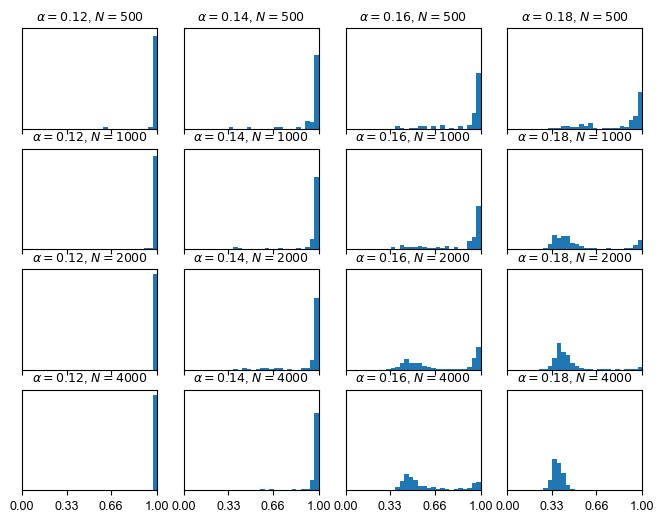
\includegraphics[clip=true,width=\columnwidth]{../ej1_histograma.png}
  \caption{}
   \label{fig:ej1_histograma}
\end{figure}

\section*{Ejercicio 2}

Se simuló la dinámica de una red de Hopfield en presencia de ruido, utilizando la regla de actualización estocástica
\[ Pr(s_i(t + 1) = \pm1) = \frac{\exp(\pm\beta h_i(t))}{\exp(\beta h_i(t)) + \exp(-\beta h_i(t))}, \]
donde \( h_i(t) = \sum_{j=1}^{N} w_{ij}s_j(t) \). Para esta simulación, se empleó dimensión \( N = 4000 \) y \( p = 40 \) patrones, resultando en un valor de \( \alpha = p/N = 0.01 \), cercano a cero. Se exploraron temperaturas \( T = \frac{1}{\beta} \) variando desde $0.1$ hasta $2$ en incrementos de $0.1$.

Se realizaron $p$ simulaciones empleando como condición inicial cada uno de los patrones \( \xi_i^\mu \). La regla de actualización se aplicó iterativamente diez veces en cada sitio de la red. A partir de estas iteraciones, se calculó el overlap medio, definido como:
\[ m^\mu = \frac{1}{N} \sum_{j=1}^{N} \langle S_j(t) \rangle \xi_j^\mu, \]
donde el promedio \( \langle \ldots \rangle \) se calculó sobre la dinámica.

En la figura \ref{fig:ej2_overlap_vs_T} se grafica el overlap medio en función de la temperatura. Los resultados muestran el comportamiento esperado con un overlap medio \( m^\mu \) igual a 1 para \( T = 0 \), de acuerdo con los resultados del ejercicio previo. A medida que la temperatura aumenta, el overlap medio disminuye progresivamente, lo cual está de acuerdo con la teoría. No obstante, en lugar de anularse completamente a \( T = 1 \), el overlap medio mantuvo un valor residual y continuó disminuyendo para temperaturas superiores. Esto puede deberse al tamaño finito del sistema.

\begin{figure}[h]
  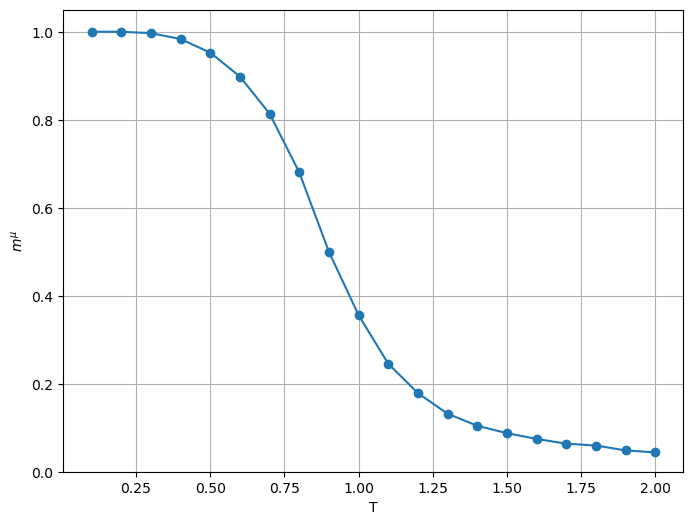
\includegraphics[clip=true,width=\columnwidth]{../ej2_overlap_vs_T.png}
  \caption{}
   \label{fig:ej2_overlap_vs_T}
\end{figure}





\onecolumngrid


\section*{Apéndice}
A continuación se desarrolla el código empleado durante este trabajo implementado en Python.




\begin{lstlisting}[language=Python]
    
    ### Ejercicio 1
    #Import libraries
    import numpy as np
    import matplotlib
    import matplotlib.pyplot as plt
    
\end{lstlisting}

\bibliography{Chehade_practica_6.bib}

\end{document}





